%%%%%%%%%%%%%%%%%%%%%%%%%%%%%%%%%%%%%%%%%%

\chapter{Commissioning of the nEDM apparatus}\label{chap:nEDM_commissioning_dec2022}

%%%%%%%%%%%%%%%%%%%%%%%%%%%%%%%%%%%%%%%%%%

Engineering run Dec 2022

%%%%%%%%%%%%%%%%%%%%%%%%%%%%%%%%%%%%%%%%%%

\section{Description of experimental setup (2022)}

%%%%%%%%%%%%%%%%%%%%%%%%%%%%%%%%%%%%%%%%%%

Refer user to Chap.~\ref{chap:LANL_nEDM}

Copper guides downstream of switcher

NiP coated electrodes

Experimental control discussed in Chap.~\ref{chap:daq}

%%%%%%%%%%%%%%%%%%%%%%%%%%%%%%%%%%%%%%%%%%

\section{Fill time measurement}

%%%%%%%%%%%%%%%%%%%%%%%%%%%%%%%%%%%%%%%%%%

 \begin{figure}
    \centering
    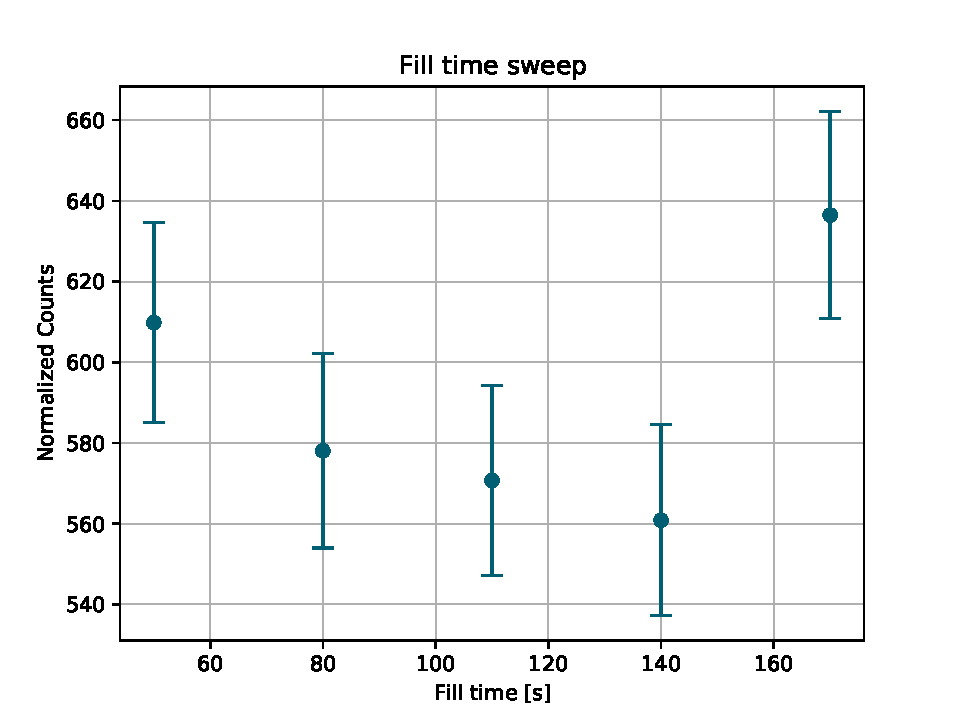
\includegraphics[width=0.6\textwidth]{figures/2022_fill_sweep.pdf}
    \caption
     {Fill-and-dump measurement in the 2022 nEDM apparatus. \qty{100}{s} preload with \qty{30}{s} storage}
    \label{fig:2022_fill_time_sweep}
\end{figure}

Fill time sweep. Normalized to West gate valve. Trying to see if that helps UCN counts (it does not)

%%%%%%%%%%%%%%%%%%%%%%%%%%%%%%%%%%%%%%%%%%

\section{Storage measurement}

%%%%%%%%%%%%%%%%%%%%%%%%%%%%%%%%%%%%%%%%%%

\begin{figure}
\centering
%subfigure width gets "multiplied" by includegraphics width
\begin{subfigure}{.5\textwidth} 
  \centering
  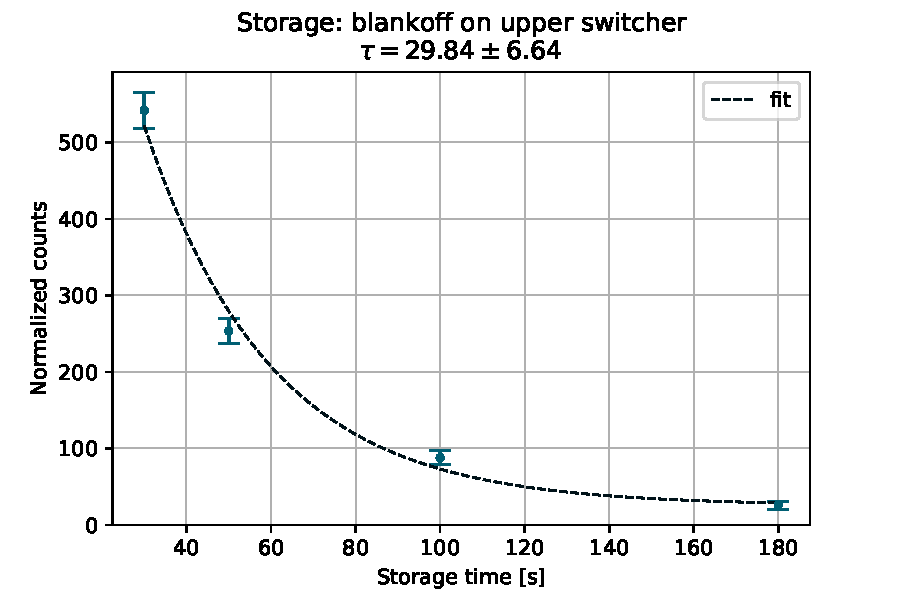
\includegraphics[width=\textwidth]{figures/store_blankoff_fit.pdf}
  \caption{}\label{subfig:2022_storage_blankoff}
\end{subfigure}%DO NOT REMOVE THIS '%'
\begin{subfigure}{.5\textwidth}
  \centering
  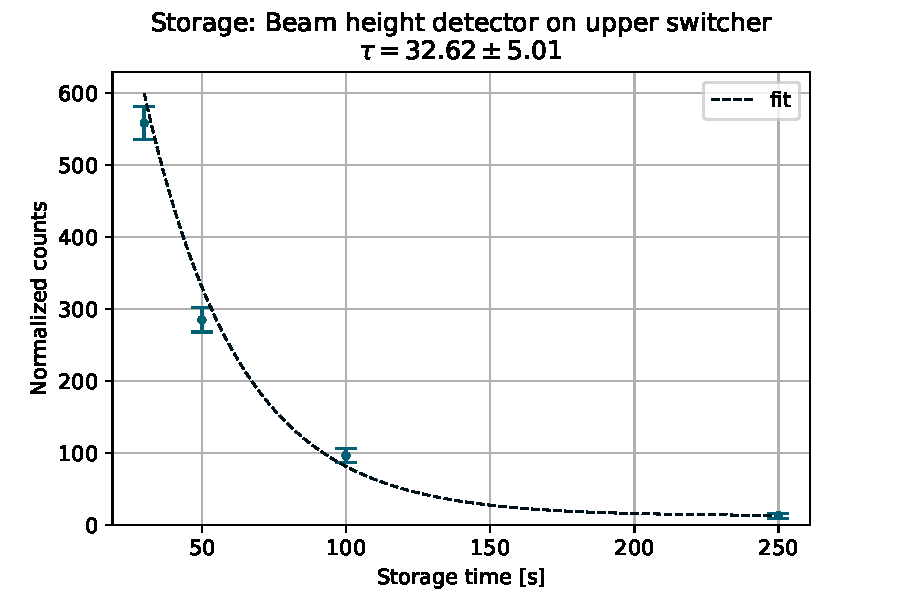
\includegraphics[width=\textwidth]{figures/store_with_beam_height_det_fit.pdf}
  \caption{}\label{subfig:2022_storage_beam_height_det}
\end{subfigure}
\caption
    [UCN storage time measurement in the lower precession cell of the apparatus fit with a single exponential of the form $A \times \exp(-t/\tau) + C$. \textbf{(\subref{subfig:2022_storage_blankoff})} and \textbf{(\subref{subfig:2022_storage_beam_height_det})} differ in terms of where \ucn are directed on the upper switcher.]
    {UCN storage time measurement in the lower precession cell of the apparatus fit with a single exponential of the form $A \times \exp(-t/\tau) + C$. \textbf{(\subref{subfig:2022_storage_blankoff})} and \textbf{(\subref{subfig:2022_storage_beam_height_det})} differ in terms of where \ucn are directed on the upper switcher. \textbf{(\subref{subfig:2022_storage_blankoff})} terminates the upper switcher to a stainless steel blankoff, and \textbf{(\subref{subfig:2022_storage_beam_height_det})} terminates to a beam height \BZnS \ucn detector.}
\label{fig:2022_ucn_storage}
\end{figure}

Load against the closed cell valve to try to see if neutrons get lost there. Then immediately turn the switcher and check guide dump counts are $4350(65)$.

%%%%%%%%%%%%%%%%%%%%%%%%%%%%%%%%%%%%%%%%%%

\subsection{Guide storage measurement}\label{sec:guide_storage_measurement}

%%%%%%%%%%%%%%%%%%%%%%%%%%%%%%%%%%%%%%%%%%

Guide storage measurement. Trying to track down UCN loss source.  Upper switcher kept at steel blank-off. Discuss lifetime change when cell valve is open

\begin{figure}
\centering
%subfigure width gets "multiplied" by includegraphics width
\begin{subfigure}{.5\textwidth} 
  \centering
  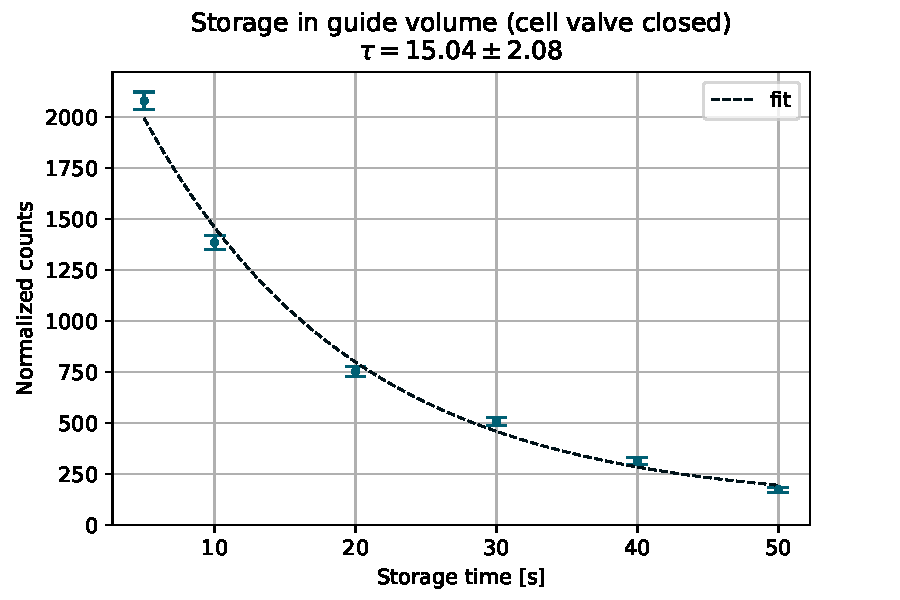
\includegraphics[width=\textwidth]{figures/store_valve_closed_fit.pdf}
  \caption{}\label{subfig:2022_guide_storage_cell_closed}
\end{subfigure}%DO NOT REMOVE THIS '%'
\begin{subfigure}{.5\textwidth}
  \centering
  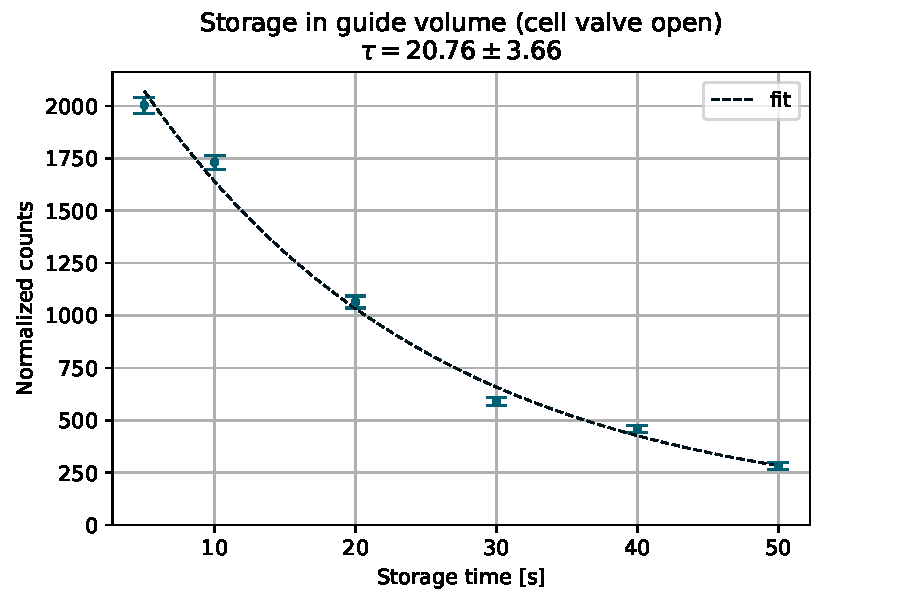
\includegraphics[width=\textwidth]{figures/store_valve_open_fit.pdf}
  \caption{}\label{subfig:2022_guide_storage_cell_open}
\end{subfigure}
\begin{subfigure}{\textwidth}
    \vspace{\baselineskip}
  \centering
  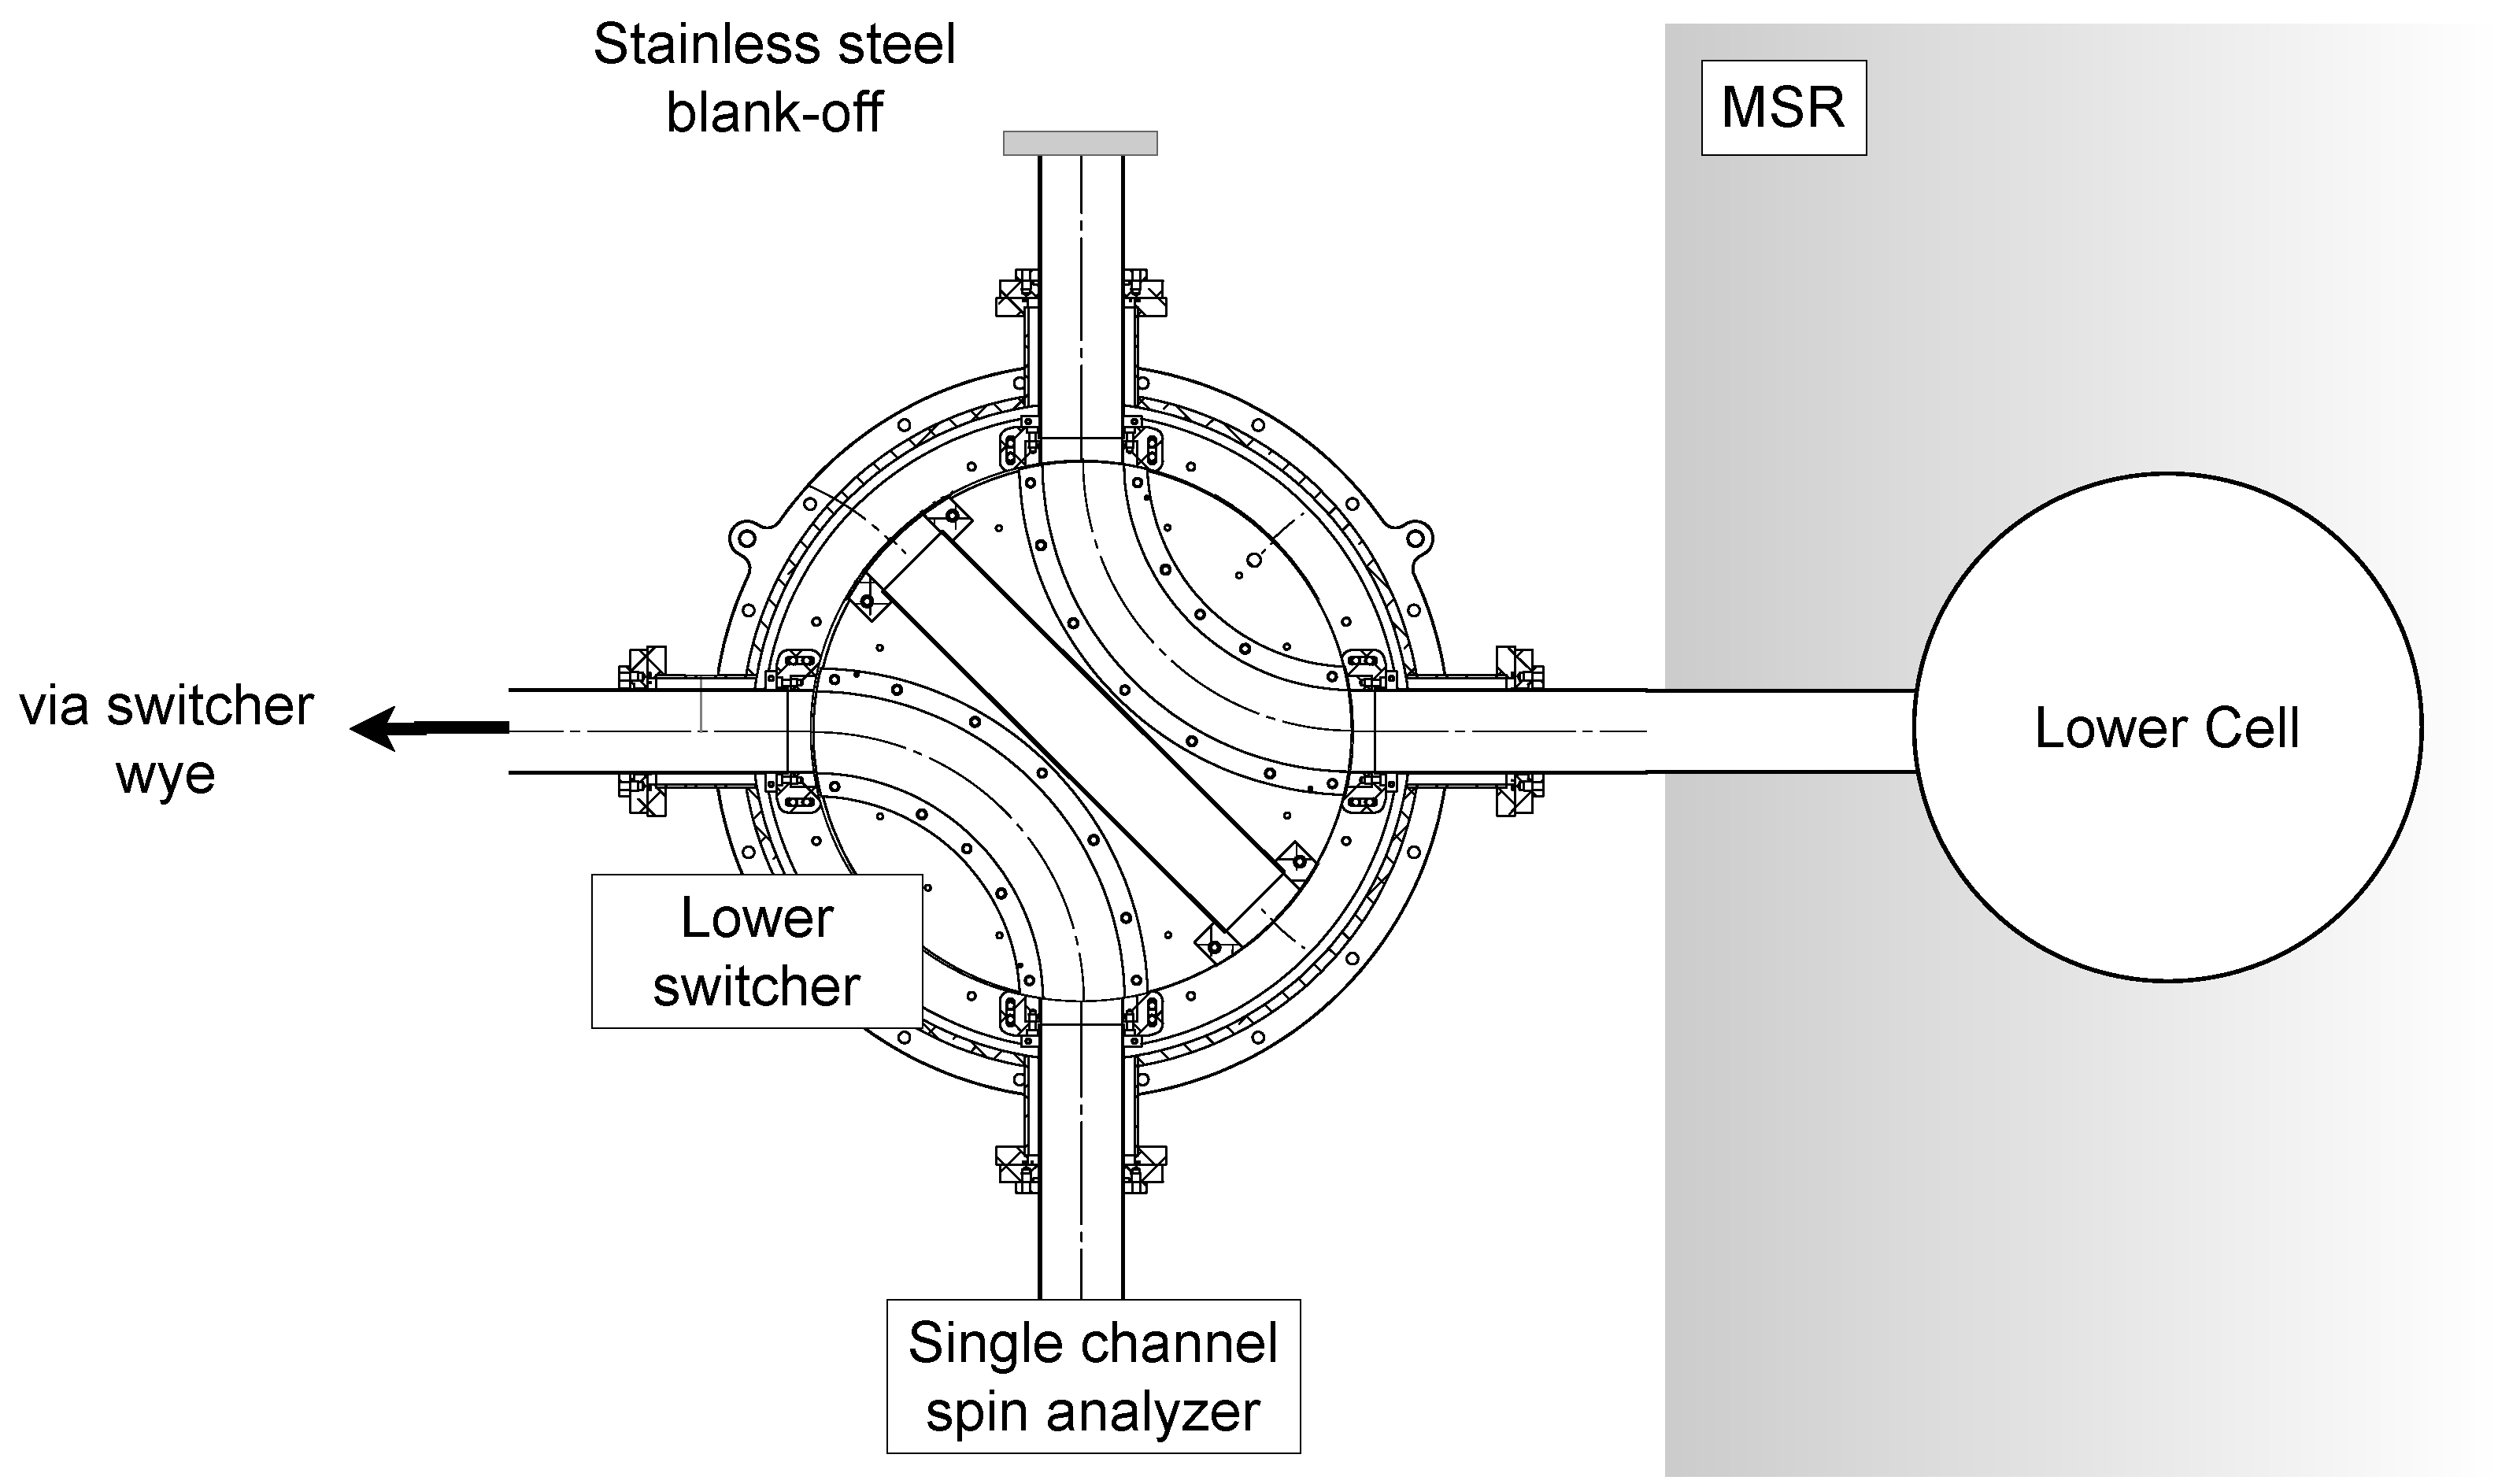
\includegraphics[width=0.8\textwidth]{figures/guide_upstream_storage.pdf}
  \caption{}\label{subfig:2022_guide_storage_schematic}
\end{subfigure}
\caption
    [Storage measurement described in Sec.~\ref{sec:guide_storage_measurement}, where UCN were stored in the guides between the lower switcher and lower cell as depicted in \textbf{(\subref{subfig:2022_guide_storage_schematic})}.]
    {Storage measurement described in Sec.~\ref{sec:guide_storage_measurement}, where UCN were stored in the guides between the lower switcher and lower cell as depicted in \textbf{(\subref{subfig:2022_guide_storage_schematic})}. \textbf{(\subref{subfig:2022_guide_storage_cell_closed})} UCN were stored in the guide volume between a stainless steel blank-off on the switcher and the closed cell valve. \textbf{(\subref{subfig:2022_guide_storage_cell_open})} The cell valve was open, so UCN were stored in the chamber as well as the guide volume.}
\label{fig:2022_ucn_guide_storage}
\end{figure}


%%%%%%%%%%%%%%%%%%%%%%%%%%%%%%%%%%%%%%%%%%

\section{Single arm spin analyzer benchmark}

%%%%%%%%%%%%%%%%%%%%%%%%%%%%%%%%%%%%%%%%%%


\begin{figure}
\centering
%subfigure width gets "multiplied" by includegraphics width
\begin{subfigure}{.5\textwidth} 
  \centering
  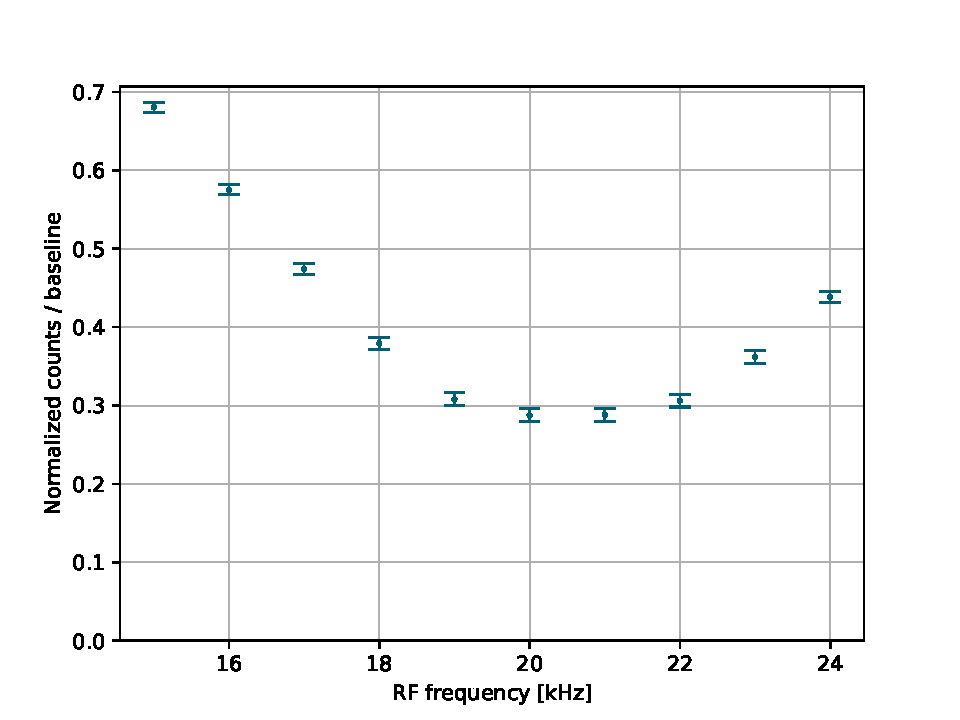
\includegraphics[width=\textwidth]{figures/2022_single_arm_spin_flip_eff.pdf}
  \caption{}\label{subfig:2022_single_arm_eff}
\end{subfigure}%DO NOT REMOVE THIS '%'
\begin{subfigure}{.5\textwidth}
  \centering
  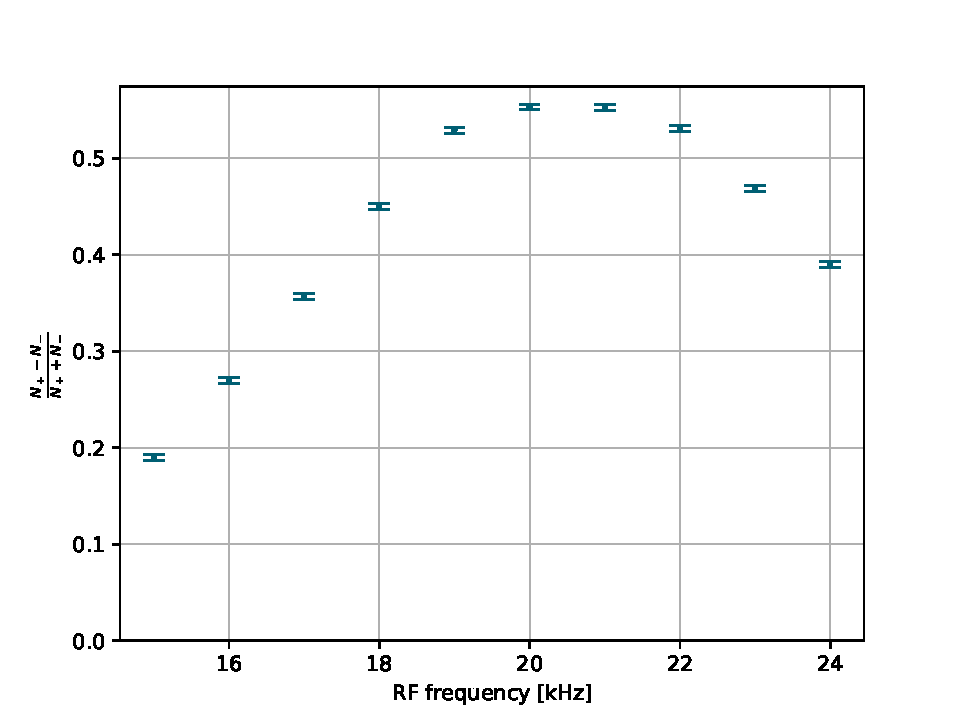
\includegraphics[width=\textwidth]{figures/2022_single_arm_spin_flip_asymmetry.pdf}
  \caption{}\label{subfig:2022_single_arm_asym}
\end{subfigure}
\caption
    {\textbf{(\subref{subfig:2022_single_arm_eff})} Single arm spin flipper efficiency as a function of the RF frequency measured on the North beamline in 2022. The count rate on the y-axis is normalized to the West Gate valve monitor, then divided by the baseline count rate with the spin flipper off. For $\text{Amp}=\qty{10}{Vpp}$, the minimum at \qty{20}{kHz} is 0.28. \textbf{(\subref{subfig:2022_single_arm_asym})} The same data replotted in terms of asymmetry}
\label{fig:2022_single_arm_asymmetry}
\end{figure}

Tuning spin flipper (see Fig.~) in flow through mode. Note the contrast and asymmetry. Upper switcher pointed at detector

Comparison of various configurations of holding field coils of single arm vs polarizer in vs out to see how many UCN we are missing. Same procedure each time, with a \qty{100}{s} preload against the NGV, before opening and flowing directly through the lower switcher to spin analyzer. Upper switcher set to beam height detector. Normalized the WGV as usual.

Make a table!!

Foil out: \qty{3404(24)}{UCN\per s}. Beam height: \qty{3657(26)}{UCN\per s}

Foil in (holding field coils OFF): \qty{2747(20)}{UCN\per s}. Beam height: \qty{3836(28)}{UCN\per s}

Foil in (holding field coils nominal): \qty{2744(20)}{UCN\per s}. \qty{3825(28)}{UCN\per s}

%%%%%%%%%%%%%%%%%%%%%%%%%%%%%%%%%%%%%%%%%%

\section{Asymmetry measurements}

%%%%%%%%%%%%%%%%%%%%%%%%%%%%%%%%%%%%%%%%%%

100s preload, 50s fill, 30s storage. RF doublet pairs, toggling every 10 - 15 seconds depending on the run. Second integration period typically shorter, so worse statistics


\begin{table}
\centering
\caption
[Measured asymmetry $A_i$ for various configurations of the $B_0$ and transport coils.]
{Measured asymmetry $A_i$ for various configurations of the $B_0$ and transport coils. $i$ refers to the integration period during the cell dump period for which the asymmetry is calculated. The currents applied to the outer $B_0$ coils (the top 2 and bottom 2 octagons), $B_0$ coils (the middle 4 octagons), and the transport coils are listed. The filling time was \qty{50}{s} and the storage time was \qty{30}{s}.}\label{tb:t1_2022_measurements}
\begin{tabular}{
    S[table-format = 2.0]
    S
    S
    c
    S[table-format = 1.2(2)]
    S[table-format = 1.2(2)]
    S[table-format = 1.2(2)]
}
\toprule
{$\sim\vv{B_0}$} 	& {$B_0$ inner}	& {$B_0$ outer} & {Transport coils} & {$A_1$} & {$A_2$} & {$A_3$}\\
{[\unit{\micro\tesla}]} 	& {[mA]}	& {[mA]} & {out $\triangleright$ in [mA]} & {} & {} & {}\\
\midrule
1 & 3.5 & 6.3 & {$91\triangleright 23.4 \triangleright 13.5 \triangleright 10.98$} & 0.02(5) & -0.01(14) & 0.03(14) \\
18 & 56 & 100 & {$91\triangleright 70\phantom{.0} \triangleright 81\phantom{.0} \triangleright 105\phantom{.0}$} & 0.00(3) & 0.00(13) & 0.01(7) \\
-1 & -3.5 & -6.3 & {$91\triangleright 23.4 \triangleright 13.5 \triangleright 10.98$} & 0.00(3) & -0.06(11) & 0.02(5) \\
-10 & -36 & -63 & {$91\triangleright 77.2 \triangleright 89.1 \triangleright 109\phantom{.0}$} & -0.02(3) & -0.02(10) & 0.00(5) \\
\bottomrule
\end{tabular}
\end{table}


%%%%%%%%%%%%%%%%%%%%%%%%%%%%%%%%%%%%%%%%%%

\section{Discussion}

%%%%%%%%%%%%%%%%%%%%%%%%%%%%%%%%%%%%%%%%%%

Refer to simulation. Can be any number of issues. Transport coils into the MSR. Magnetized components that are saturated on the beamline.